\documentclass[a4paper,10pt]{article}
%\usepackage[latin1]{inputenc} % Paquetes de idioma
\usepackage[utf8]{inputenc} % Paquetes de idioma (Este encoding toma acentos :) )
\usepackage[spanish]{babel} % Paquetes de idioma
\usepackage{graphicx} % Paquete para ingresar gráficos
\usepackage{grffile}
\usepackage{hyperref}
\usepackage{fancybox}
\usepackage{amsmath}
\usepackage{amsfonts}
\usepackage{listings}
\usepackage{float}
% Paquetes de macros de Circuitos
%\usepackage{pstricks}
\usepackage{tikz}
% Encabezado y Pié de página
\usepackage{fancyhdr} % Paquete para encabezados y pie de página
\pagestyle{fancy} % Sin esta línea no se imprimiría el encabezado en todas las páginas

\fancyhf{} %  Borra el encabezado anterior (Por defecto escribe el títutlo de la sección en la que se encuentra la hoja
\setlength{\headheight}{22.55pt}
\fancyhead[L]{
	{\textsf{Facultad de Ingenier\'ia $-$ Universidad de Buenos Aires \\ 66.44 Instrumentos Electrónicos}}
}
%\addtocounter{page}{5}
\fancyhead[R]{\thepage}

\renewcommand{\footrulewidth}{0.4pt} % Ajusta el tamaño de las líneas separadoras en el pié de página
\renewcommand{\headrulewidth}{0.4pt} % Ajusta el tamaño de las líneas separadoras en el encabezado

\fancyfoot[L]{
	{\textsf{Trabajo Pr\'actico N$^{\circ}4$}: Mediciones de impedancias} \\
	{\textsf{Integrantes: Eduardo Sanchez, Francisco Soler}}
	}
		

% Carátula del Trabajo
\title{ \author{} % Lo pongo para que el warning no moleste :p
\setlength{\unitlength}{1cm} %  Especifica la unidad de trabajo
\thispagestyle{empty}

\begin{picture}(18,0)
\put(0,0){
\includegraphics[width=1.5cm, height=3cm]{Logo1.png}}

\put(10.5,0){
\includegraphics[width=3cm, height=3cm]{Logo2.png}}

\end{picture}
\\[1.5cm]
\begin{center}
	\textbf{{\Huge Facultad de Ingenier\'ia \\ Universidad de Buenos Aires}}\\[2cm]
	{66.44 Instrumentos Electrónicos}\\[0.5cm]
	{Trabajo Pr\'actico N$^{\circ}3$: Mediciones de impedancias}\\[2.5cm]
\end{center}

\begin{flushleft}
	\textbf{Integrantes:} \\[1cm]

	\begin{tabular}{|c|c|c|}
		\hline
		\textbf{\normalsize Padr\'on} & \textbf{\normalsize Nombre} & \textbf{\normalsize Email} \\
		\hline
		\normalsize 92903 & \normalsize Sanchez, Eduardo Hugo & \normalsize hugo\_044@hotmail.com \\
		\hline
		\normalsize 91227 & \normalsize Soler, Jos\'e Francisco & \normalsize francisco.\_tw@hotmail.com \\
		\hline
		\normalsize xxx & \normalsize Wawrynczak, Claudio  & \normalsize claudiozak@gmail.com \\
		\hline
	\end{tabular}
\end{flushleft}
\date{} % Hace que no se imprima la fecha en la cual se compilo el .tex
 }

\begin{document}
	\maketitle % Hace que el título anterior sea el principal del documento
	\newpage

	\tableofcontents % Esta línea genera un indice a partir de las secciones y 
					% subsecciones creadas en el documento
	\newpage
	

	\section{Objetivo}
	
	\indent	El objetivo del presente trabajo práctico es determinar el 
	comportamiento de distintas funcionalidades del osciloscopio 
	tales como la FFT y el nivel ruido propio de cada osciloscopio de acuerdo a
	su ancho de banda. Finalmente se mide el nivel de ruido generado por una 
	fuente de tensi\'on del laboratorio. 

	\newpage
	\section{Desarrollo}
	
\indent Para llevar a cabo las mediciones, se utilizan los siguientes
		instrumentos:
		\begin{itemize}
			\item Un generador de señales senoidales.
			\item Una fuente de tensi\'on.
			\item Tres osciloscopios de diferente ancho de banda:RIGOL DS1102E (
			$BW=100MHz$), RIGOL DS1104B ($BW=200MHz$) y RIGOL DS1302CA (
			$BW=300MHz$).
			\item La punta Rigol RP3300.
			\item Cable coaxil para realizar las distintas conexiones entre 
			instrumentos.
		\end{itemize}
		
	\subsection{Medición 1 - Comportamiento FFT}
	\indent En esta medición se compara el comportamiento de la funcionalidad
	FFT dispuesta en el osciloscopio utilizando cuatro tipos de ventanas de 
	muestreo diferente: rectangular, Hanning, Hamming y Blackman.\\
	\indent El banco de medici\'on est\'a compuesto por el osciloscopio (RIGOL 
	DS1302CA) cuya impedancia de entrada est\'a seleccionada en $50\Omega$ para 
	que est\'e adaptado al cable coaxil que lo conecta con el generador de 
	señales. La frecuencia de la senoidal utilizada debe estar contenida en el 
	ancho de banda del conjunto punta-osciloscopio. \\
	\indent Se utilizarán 3 frecuencias contiguas de forma tal de observar cómo
	se modifica la amplitud del pico de la sinc observada (dependiendo del tipo 
	de ventana, queda recortado cuando no cae en un punto de medición de la FFT)
	. \\
	\indent En las siguientes figuras, la frecuencia de la señal de la imagen de
	la izquierda corresponde a $11MHz$, la del medio a $11,7MHz$ y la de la 
	derecha a $11,9MHz$.\\
	\indent En la figura \ref{img001} se puede observar que efectivamente el 
	pico de la señal queda recortado. Logrando una diferencia de altura de la 
	señal en unos $1.5dB$.

	\begin{figure}[!htb]
		\centering
		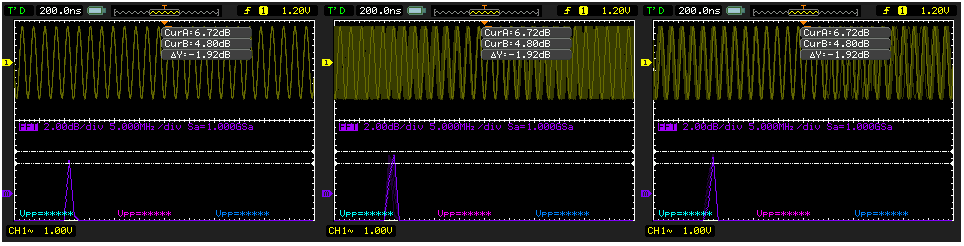
\includegraphics[width=12cm]
		{Imagenes/RectangularWindow.png}
		\caption{FFT de una señal senoidal utilizando una ventana Cuadrada.}
		\label{img001}
	\end{figure}

	\indent En la figura \ref{img002} se puede observar que, a diferencia
	de utilizar una ventana cuadrada, con la Hanning el pico de la sinc no 
	disminuye en amplitud, por ende el pico siempre es el mismo.

	\begin{figure}[!htb]
		\centering
		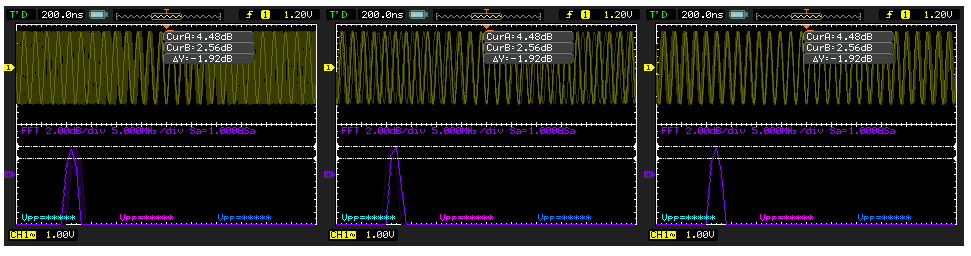
\includegraphics[width=12cm]
		{Imagenes/HanningWindow.png}
		\caption{FFT de una señal senoidal utilizando una ventana Hanning.}
		\label{img002}
	\end{figure}

	\indent En la figura \ref{img003} se puede observar que con la ventana 
	Hamming no hay grandes diferencias con la Hanning, simplemente se observa 
	un lóbulo levemente más angosto.

	\begin{figure}[!htb]
		\centering
		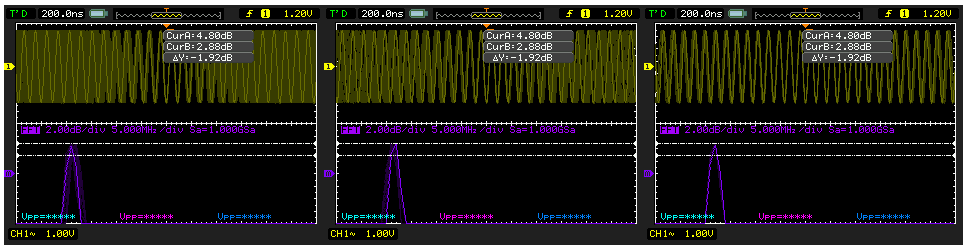
\includegraphics[width=12cm]
		{Imagenes/HammingWindow.png}
		\caption{FFT de una señal senoidal utilizando una ventana Hamming.}
		\label{img003}
	\end{figure}

	\indent En la figura \ref{img004} se puede observar que con la ventana 
	Blackman no hay grandes diferencias con las dos anteriores, simplemente se 
	observa que el lóbulo es levemente más ancho y que el pico está en una 
	altura menor, aproximadamente en $2,90dB$ mientras que las otras están en 
	$4,80dB$.

	\begin{figure}[!htb]
		\centering
		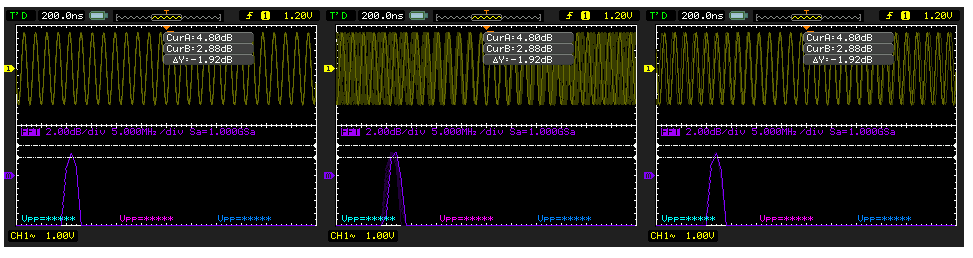
\includegraphics[width=12cm]
		{Imagenes/BlackmanWindow.png}
		\caption{FFT de una señal senoidal utilizando una ventana Blackman.}
		\label{img004}
	\end{figure}
	
	\indent Estas mediciones concuerdan con el manual del fabricante: la ventana 
	rectangular es la de menor ancho de l\'obulo (y por ende la de mejor 
	resoluci\'on de frecuencia) pero tambi\'en es la que ofrece peor 
	resoluci\'on en magnitud. La ventana de Hanning tiene una mejor resoluci\'on
	en magnitud que la rectangular, la de Hamming tiene una resoluci\'on en 
	magnitud similar a la de Hanning pero mejora en frecuencia ya que tiene un 
	ancho de l\'obulo menor. Respecto de la ventana de Blackman, \'esta es la 
	que posee mejor resoluci\'on de magnitud ya que es la que menos var\'ia al 
	cambiar la frecuencia aunque es la de mayor ancho de l\'obulo. \\
	\indent Esta funcionalidad no es \'util si las incertezas que se deben 
	obtener en la medici\'on de amplitud deben ser menores a $1,5dB$ (cota que 
	se adopta del peor caso).

	\subsection{Medición 2 - Ruido interno del osciloscopio}
	\indent En esta medici\'on, se pretende obtener el piso de ruido existente 
	en osciloscopios de diferente ancho de banda. Para ello se conecta por 
	separado a cada uno de los 3 osciloscopios disponibles una carga de 
	$50\Omega$ para observar el ruido que genera internamente cada osciloscopio.
	Dado que solo se analiza el ruido en un determinado intervalo de tiempo (una
	aproximaci\'on al valor real), es importante que las bases de tiempos sean 
	iguales en los 3 osciloscopios de manera de poder realizar un an\'alisis 
	comparativo. \\
	\indent En la Figura \ref{img005}, se observa el nivel de ruido del 
	osciloscopio RIGOL DS1102E cuyo ancho de banda es de $100MHz$. Resulta 
	importante conocer la potencia del ruido para poder luego obtener otros 
	par\'ametros como la relaci\'on se\~nal a ruido, $SNR$.\\
	\indent Su valor de amplitud RMS es de $V_{RMS(100Mhz)}=179\mu V \pm87\mu V$
	. Es importante advertir que la incerteza especificada por el fabricante 
	(del $4\%$ para la escala de $2mV/div$, es decir unos $7\mu V$) es mucho 
	menor que el error de cuantizaci\'on del osciloscopio ($80\mu V$).
		\begin{figure}[!htb]
			\centering
			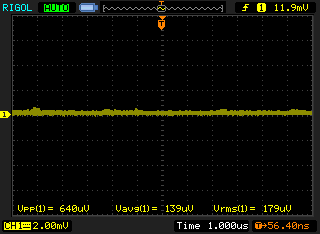
\includegraphics[width=5cm]
			{Imagenes/Ruido100Mhz.png}
			\caption{Ruido presente a la entrada del osciloscopio RIGOL DS1102E}
			\label{img005}
		\end{figure}
		
	\indent En la Figura \ref{img006}, se observa el nivel de ruido del 
	osciloscopio RIGOL DS1104B cuyo ancho de banda es de $200MHz$. \\
	\indent Su valor de amplitud RMS es de $V_{RMS(200Mhz)}=367\mu V \pm95\mu V$
	Nuevamente el error de cuantizaci\'on ($80\mu V$) es bastante mayor al de la
	incerteza del osciloscopio ($15\mu V$)
		\begin{figure}[!htb]
			\centering
			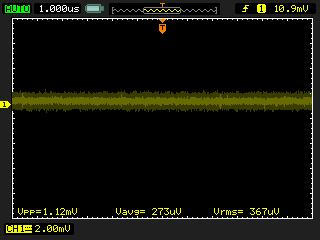
\includegraphics[width=5cm]
			{Imagenes/Ruido200Mhz.png}
			\caption{Ruido presente a la entrada del osciloscopio RIGOL DS1104B}
			\label{img006}
		\end{figure}
		
	\indent En la Figura \ref{img007}, se observa el nivel de ruido del 
	osciloscopio RIGOL DS1302CA cuyo ancho de banda es de $300MHz$. \\
	\indent Su valor de amplitud RMS es de $V_{RMS(300Mhz)}=113\mu V \pm85\mu V$
	En este caso el error de cuantizaci\'on ($80\mu V$) es el mismo que antes y 
	la incerteza del osciloscopio es de $5\mu V$.
		\begin{figure}[!htb]
			\centering
			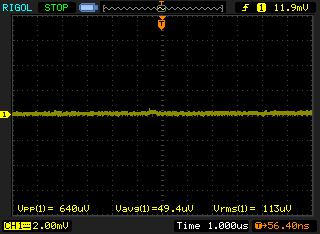
\includegraphics[width=5cm]
			{Imagenes/Ruido300Mhz.png}
			\caption{Ruido presente a la entrada del osciloscopio RIGOL DS1302CA
			}
			\label{img007}
		\end{figure}\\
	\indent En principio se puede suponer que el ruido presente en la entrada 
	del osciloscopio es ruido blanco. Con lo cual, al tener componentes en todo 
	el espectro de frecuencias, al utilizar osciloscopios de mayor ancho de 
	banda la potencia de este ruido deber\'ia aumentar. Esto se puede ver en los
	primeros dos casos, el osciloscopio de $100MHz$ tiene un nivel de ruido 
	menor al de $200MHz$. \\
	\indent No obstante, esto no ocurre en el caso del osciloscopio de $300MHz$ 
	cuyo nivel de ruido es el menor de todos. Seguramente esto se deba a la 
	tecnolog\'ia misma del osciloscopio que se adec\'ua para no tener un nivel 
	de ruido elevado y por ende un osciloscopio de menores prestaciones. \\
	\indent A modo de comparación, en la tabla \ref{tab001} se muestran todos 
	los valores medidos.
	
	\begin{table}[!htp]
		\centering
		\begin{tabular}{|c|c|c|c|c|c|}
			\hline
    		Modelo & Error de cuant.& Incerteza (Vrms) & V pap & V avg & V rms\\
			\hline
			DS1204B & $80~\mu\text{V}$& $95~\mu\text{V}$ & $1.12~\text{mV}$ & 
			$273~\mu\text{V}$ & $367~\mu\text{V}$ \\
			\hline 
			DS1102E & $80~\mu\text{V}$& $87~\mu\text{V}$ & $640~\mu\text{V}$ & 
			$139~\mu\text{V}$ & $179~\mu\text{V}$ \\
			\hline
			DS1302CA & $80~\mu\text{V}$& $85~\mu\text{V}$ & $640~\mu\text{V}$ & 
			$49.4~\mu\text{V}$ & $113~\mu\text{V}$ \\
			\hline
		\end{tabular}
		\caption{Comparación de mediciones entre los distintos osciloscopios} 
		\label{tab001}
	\end{table}
	Del cuadro puede observarse que el osciloscopio de mejores prestaciones es 
	el RIGOL-DS1302CA ya que posee mayor ancho de banda y un nivel de ruido 
	menor que el resto de los osciloscopios.
			
	\subsection{Medición 3 - Ruido de la fuente}
	\indent En esta secci\'on se mide el ruido presente en una fuente de $5.2V$.
	La entrada del osciloscopio (se utiliza el modelo DS1102E ya que sus 
	prestaciones permiten realizar la medic\'on adecuadamente) se conecta en AC 
	y se observa la se\~nal resultante. En la Figura \ref{img008} puede 
	observarse la respuesta temporal y el espectro de dicha se\~nal (para 
	diferenciar los or\'igenes de los ruidos se utiliza como referencia el 
	ruido generado por el osciloscopio).

		\begin{figure}[!htb]
			\centering
			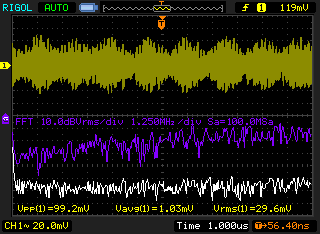
\includegraphics[width=5cm]
			{Imagenes/RuidoFuente.png}
			\caption{Ruido generado por una fuente de tensi\'on}
			\label{img008}
		\end{figure}
	\indent Del gr\'afico puede observarse que aproximadamente la diferencia 
	entre el ruido de base del que aporta la fuente es de $40dB$.\\ 
	El valor de amplitud RMS del ruido (tanto de la fuente como del osciloscopio
	) es de $V_{RMS}=29,6mV \pm 1,3mV $. En este caso el error de cuantizaci\'on
	($80\mu V$) es mucho menor al de la incerteza especificada ($4\%$ de la 
	lectura, es decir, $1,2mV$). Por otra parte es mucho mayor al piso ruido 
	propio del osciloscopio. La diferencia en decibeles entre estos ruidos 
	est\'a dada por la siguiente relaci\'on 
	$$20\log(\frac{V_{RMS(medido)}}{V_{RMS(ruido~ osciloscopio)}})$$.
	$$20\log(\frac{29,6mV \pm 1,3mV}{367\mu V \pm95\mu V})=38dB \pm 0,3dB$$
	\indent Lo cual se aproxima razonablemente al valor observado en pantalla. 
	Debe notarse que si bien la incerteza del valor RMS de la se\~nal de ruido 
	es alta ($25\%$ del valor de referencia) la incerteza en dB es mucho menor 
	($0,8\%$) debido a las caracter\'istica de la funci\'on logaritmica. 
%FRANNNNNNNNNNNNNNNNNNNNNNNNNNNNNNNNNNNNNNNNNNNNNNNNNNNNNNNNNNNNNNNNNNNNNNNNNNNNNNNNNNNNNNNNNNNNN esto tiene que ir al tp 1, así no queda super desorganizado, ya esta corregido solo copialo y pegalo.
	\subsection{Medición 4 - Tiempo de crecimiento de una compuerta}
	\indent Utilizando el osciloscopio de $300MHz$ de ancho de banda, RIGOL 
	DS1302CA, se midi\'o el retardo y tiempo de crecimiento que impone una 
	compuerta AND (del integrado 74LS08). \\
	\indent En la figura \ref{banco} se muestra el esquema de conexi\'on 
	utilizado. \\
 	\indent Como la circuitería del integrado requiere picos de corriente para 
	poder llevar la salida de un estado bajo a uno alto, es necesario conectar 
	en el terminal de alimentación un capacitor que sea capaz de entregar dicha 
	energía. Esto se debe a que el circuito está conectado a través de una línea
	de transmisión a la fuente de alimentación y el efecto de esta conexión es 
	generar retardos en la entrega de dichos picos y por ende disminuir el 
	tiempo de crecimiento de la compuerta.\\
	\indent En la Figura \ref{img009}, se puede observar las siguientes medidas 
	$$t_{delay}=8.90ns \pm0.4ns$$y  $$t_{c}=11.20ns\pm0.5ns$$. \\
	\indent La hoja de datos del fabricante indica un valor de $t_{delay}=8.ns$ 
	cuando el estado pasa de bajo a alto, lo cual coincide aproximadamente con 
	el valor obtenido. \\
	\indent De esta manera resulta importante conocer la tecnlog\'ia de 
	fabricaci\'on de estos dispositivos para conocer las limitaciones que 
	presentan en cuanto velocidad.
	
		\begin{figure}[!htb]
				\centering
				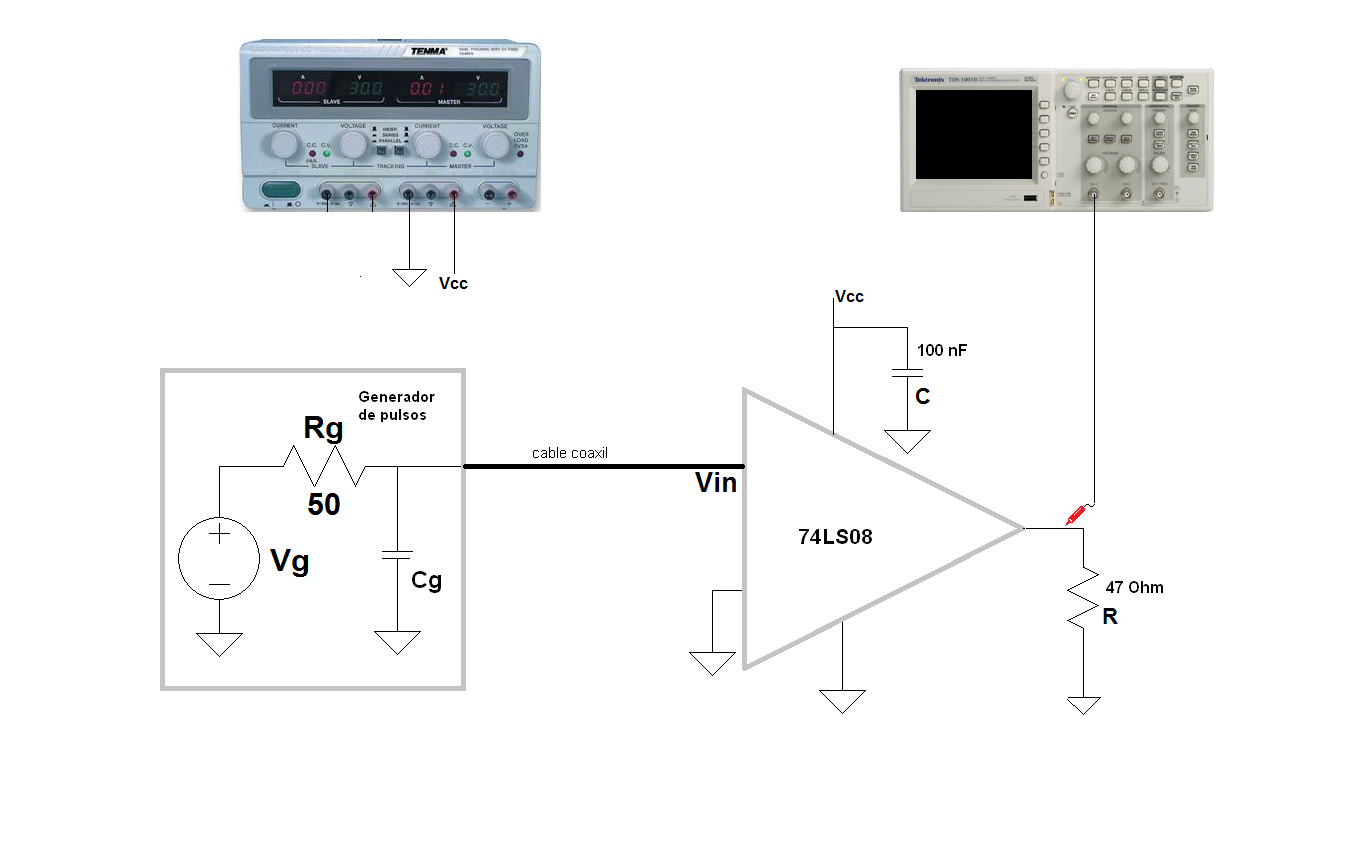
\includegraphics[width=7cm]
				{Imagenes/banco.png}
				\caption{Esquema de conexi\'on del integrado 74LS08}
				\label{banco}
			\end{figure}
		
		\begin{figure}[!htb]
			\centering
			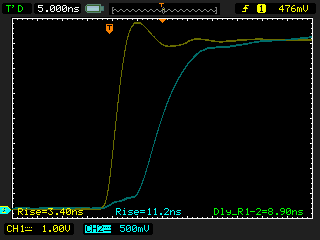
\includegraphics[width=5cm]
			{Imagenes/Risetime3.png}
			\caption{Se\~nal de entrada a la compuerta (en amarillo) y se\~nal 
			de salida (en celeste)}
			\label{img009}
		\end{figure}

	%HUGOOOOOOOOOOOOOOOOOOOOOOOOOOOOOOOOOOOOOOOOOOOOOOOOOOOOOOOOOOOOOOOOOOOOOOOOOOOOOOOOOOOOOOOOO esto va para el tp3 sino queda colgado acá
	\subsection{Medición 5 - Reflectometría}
	\indent En esta medición se calcula el largo de distintos cables, para ello
	se conecta un generador y un osciloscopio en el mismo terminal del cable. El
	generador emite un pulso y, dependiendo que impedancia está conectada el 
	otro terminal, la señal rebota con la misma fase, fase opuesta o no se 
	refleja absolutamente nada. \\
	\indent Se mide el tiempo que tarda la señal en ir y volver por el cable y,
	con dicho resultado, se calcula la velocidad de propagación sobre el mismo.
	\\
	\indent La imágenes \ref{img010}, \ref{img011} y \ref{img012} muestran tres
	tipos de adaptaciones: izquierda posee un circuito abierto; medio, adaptado;
	derecha, cortocircuito. \\

		\begin{figure}[!htb]
			\centering
			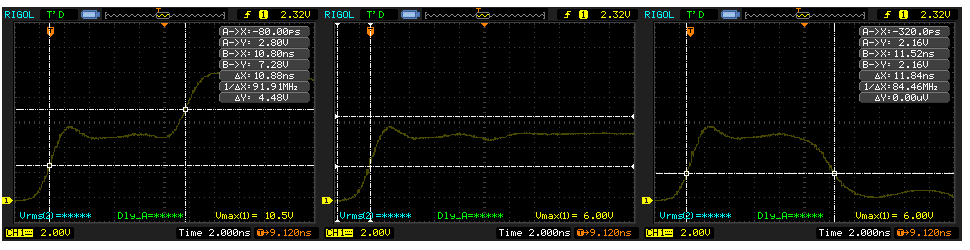
\includegraphics[width=5cm]
			{Imagenes/CableF&G.png}
			\caption{Propagación de la señal en un cable $RG-213/U$}
			\label{img010}
		\end{figure}
		\begin{figure}[!htb]
			\centering
			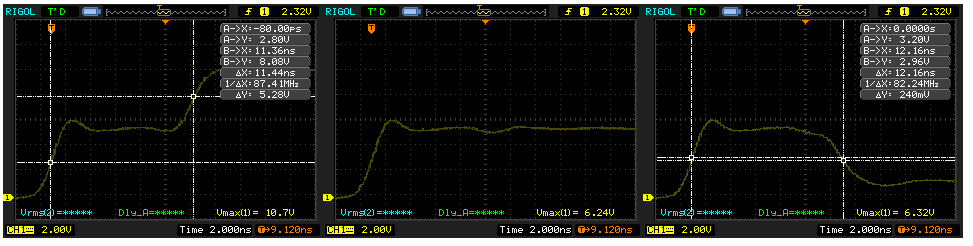
\includegraphics[width=5cm]
			{Imagenes/CableCoaxialFino.png}
			\caption{Propagación de la señal en un cable coaxial fino}
			\label{img011}
		\end{figure}
		\begin{figure}[!htb]
			\centering
			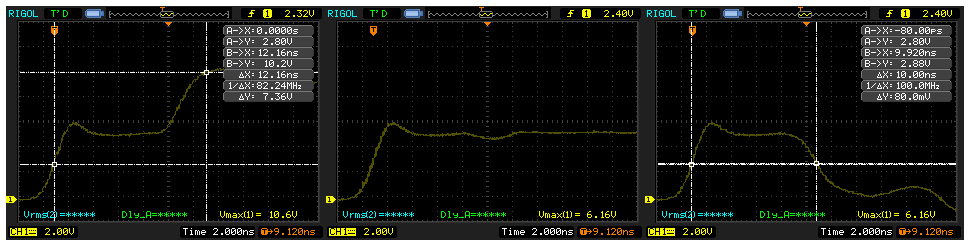
\includegraphics[width=5cm]
			{Imagenes/CableCoaxialGrueso.png}
			\caption{Propagación de la señal en un cable coaxial grueso}
			\label{img012}
		\end{figure}

	\indent La tabla \ref{tab002} muestra los distintos cables con sus 
	respectivas longitudes, tiempo y velocidad de propagación. En
	la longitud se está tomando en cuenta el largo de la $T$ utilizada para 
	conectar el osciloscopio al cable, el cual mide $18 cm$. \\
	
	\begin{table}[!htp]
		\centering
		\begin{tabular}{|c|c|c|c|}
			\hline
    		Cable & longitud total & $\tau$ & Vel propagación \\
			\hline
			F\&G RG-213/u & $1.18~\text{m}$ & $10.88\cdot~\text{c}$ & 
			$0.36~\cdot\text{c}$ \\
			\hline 
			coaxil fino & $1.24~\text{m}$ & $11.44~\mu\text{n seg}$ &
			$0.36~\cdot\text{c}$ \\
			\hline
			coaxil grueso & $1.44~\text{m}$ & $10.72~\mu\text{n seg}$ & 
			$0.45~\cdot\text{c}$ \\
			\hline
		\end{tabular}
		\caption{Comparación de velocidades de propagación entre distintos 
		tipos de cables} \label{tab001}
	\end{table}
 
	\newpage 
	\section{Conclusiones}
	Las funcionalidades del osciloscopio analizadas en este trabajo (FFT y nivel
	de ruido en relaci\'on al ancho de banda) fueron comprendidas a nivel 
	pr\'actico gracias a las experiencias realizadas en el laboratorio.\\
	\indent Por ejemplo, se concluy\'o que el ruido interno del osciloscopio no 
	depende solamente del ancho de banda del mismo (como ocurre idealmente), 
	sino también de la calidad de sus componentes. Esto se puede apreciar con el
	osciloscopio de 300MHz, que posee un ruido interno menor a los otros de 
	menor ancho de banda. \\
	\indent Respecto a la FFT, resulta una herramienta \'util si lo que se desea
	es tener una idea del espectro de la se\~nal bajo an\'alisis. Sin embargo 
	presenta una incertidumbre alta, por lo cual para mediciones de precisi\'on 
	se sugiere utilizar otro instrumento.
%	\indent El uso de la reflectometría es un muy buen método para poder 
%	determinar distintos parámetros de la línea de transmisión a medir, ya sea 
%	el estado de la misma como del largo, etc. \\
%	\indent A la hora de utilizar compuertas o cualquier circuito que requiera 
%	picos de corriente, hay que prestar mucha atención en que frecuencias se 
%	está trabajando para poder utilizar un capacitor que en dichas frecuencias 
%	posea la menor impedancia posible (que entre en resonancia el RLC 
%	equivalente). \\
\end{document}

